% !TEX TS-program = pdflatex
% !TEX encoding = UTF-8 Unicode

% This is a simple template for a LaTeX document using the "article" class.
% See "book", "report", "letter" for other types of document.

\documentclass[11pt]{article} % use larger type; default would be 10pt

\usepackage[utf8]{inputenc} % set input encoding (not needed with XeLaTeX)

%%% Examples of Article customizations
% These packages are optional, depending whether you want the features they provide.
% See the LaTeX Companion or other references for full information.

%%% PAGE DIMENSIONS
\usepackage{geometry} % to change the page dimensions
\geometry{a4paper} % or letterpaper (US) or a5paper or....
 \geometry{margin=2cm} % for example, change the margins to 2 inches all round
% \geometry{landscape} % set up the page for landscape
%   read geometry.pdf for detailed page layout information

\usepackage{graphicx} % support the \includegraphics command and options
\graphicspath{{figures/}}

% \usepackage[parfill]{parskip} % Activate to begin paragraphs with an empty line rather than an indent

%%% PACKAGES
%\usepackage{booktabs} % for much better looking tables
%\usepackage{array} % for better arrays (eg matrices) in maths
%\usepackage{paralist} % very flexible & customisable lists (eg. enumerate/itemize, etc.)
%\usepackage{verbatim} % adds environment for commenting out blocks of text & for better verbatim
%\usepackage{subfig} % make it possible to include more than one captioned figure/table in a single float
% These packages are all incorporated in the memoir class to one degree or another...
\usepackage{algorithmic}
\usepackage{algorithm}

%\floatname{algorithm}{Procedure}
\renewcommand{\algorithmicrequire}{\textbf{Input:}}
\renewcommand{\algorithmicensure}{\textbf{Output:}}

%%% HEADERS & FOOTERS
%\usepackage{fancyhdr} % This should be set AFTER setting up the page geometry
%\pagestyle{fancy} % options: empty , plain , fancy
%\renewcommand{\headrulewidth}{0pt} % customise the layout...
%\lhead{}\chead{}\rhead{}
%\lfoot{}\cfoot{\thepage}\rfoot{}

%%% SECTION TITLE APPEARANCE
%\usepackage{sectsty}
%\allsectionsfont{\sffamily\mdseries\upshape} % (See the fntguide.pdf for font help)
% (This matches ConTeXt defaults)

%%% ToC (table of contents) APPEARANCE
%\usepackage[nottoc,notlof,notlot]{tocbibind} % Put the bibliography in the ToC
%\usepackage[titles,subfigure]{tocloft} % Alter the style of the Table of Contents
%\renewcommand{\cftsecfont}{\rmfamily\mdseries\upshape}
%\renewcommand{\cftsecpagefont}{\rmfamily\mdseries\upshape} % No bold!

%%% END Article customizations

%%% The "real" document content comes below...

\title{Summaries of a few papers on mitral valve prolapse and cross-modal image registration}
\author{Stephan}
%\date{} % Activate to display a given date or no date (if empty),
         % otherwise the current date is printed

\begin{document}
\maketitle

\tableofcontents

%% RECHERCHER LE SCORE "DICE" UTILISé POUR LA SEGMENTATION

%\section{Medical imaging problems}
%\begin{itemize}
%  \item Image registration
%  \begin{itemize}
%    \item Point cloud registration
%    \begin{itemize}
%      \item Iterative Closest Point algorithm \cite{besl:icp, chen:icp}
%      \item Random Sample Consensus (RanSaC) algorithm \cite{fischler:ransac}
%      \item Cross-modal point cloud registration \cite{huang:kinect}
%    \end{itemize}
%
%    \item Intensity-based registration
%        \begin{itemize}
%           \item Electron microscopy to light microscopy \cite{acosta:intensity}
%        \end{itemize}
%    \item Cross-modal registration using image analogies
%        \begin{itemize}
%           \item Building dictionaries of features \cite{cao:analogies}
%        \end{itemize}
%  \end{itemize}
%  \item Analysis of cell images
%  \begin{itemize}
%    \item Segmentation
%    \begin{itemize}
%      \item Colour threshold and pixel adjacency
%      \item After segmentation, decision tree to classify an image segment as a cell or not a cell based on its area and elongation \cite{kan:machine}
%      \item Convolutional neural networks
%        \begin{itemize}
%           \item 2018 Data Science Bowl \cite{marks:bowl}
%        \end{itemize}
%    \end{itemize}
%    \item Tracking and constructing lineage trees
%        \begin{itemize}
%           \item Given two successive frames, classify all pairs (cell from first frame, cell from second frame) as "same cell" or "distinct cells" \cite{kan:machine}
%        \end{itemize}
%  \end{itemize}
%\end{itemize}


%  \item Decision tree to classify an image segment as a cell or not a cell based on its area and elongation;
%  \item Given two successive frames, classify all pairs (cell from first frame, cell from second frame) as "same cell" or "distinct cells";

\newpage

\section{Image registration}
  \subsection{ 3d Point set registration}
    \subsubsection{ Point set to point set: Iterative Closest Point algorithm \linebreak[4] \cite{besl:icp, chen:icp}}
An algorithm to register two sets of points. The basic principle is that it is easy to register two sets of points if the points are matched in pairs, and hard if they are not. See Algorithm \ref{algo:icp}.

\begin{algorithm}[h!]
\caption{Iterative Closest Point}
\label{algo:icp}
\begin{algorithmic}
  \REQUIRE two sets of points $X$ and $Y$; ``find closest point'' procedure; ``find best transformation'' procedure
  \ENSURE a transformation from $Y$ to $X$
  \REPEAT
    \FOR{every point $y \in Y$}
      \STATE find the point $x(y) \in X$ that is closest to $y$
    \ENDFOR
%    \STATE For every point $y \in Y$, find the point $x(y) \in X$ that is closest to $y$
    \STATE find the transformation $q$ that best maps all points in $Y$ to their image in $X$
    \STATE apply $q$ to $Y$
  \UNTIL{$\sum_{y \in Y} ||q(y)-y|| \leq$ some threshold, or number of iterations $\geq$ some threshold }
  \RETURN the transformation obtained by composing all the successive transformations
\end{algorithmic}
\end{algorithm}

%\begin{itemize}
%  \item \emph{Input:} Two sets of points $X$ and $Y$; "find closest point" procedure; "find best transformation" procedure
%  \item Loop:
%  \begin{itemize}
%    \item For every point $y \in Y$, find the point $x(y) \in X$ that is closest to $y$
%    \item Find the transformation $q$ that best maps $Y$ to $\{ x(y),\, y \in Y \}$
%    \item Apply $q$ to $Y$
%  \end{itemize}
%\end{itemize}

    \subsubsection{ Model to point set: Random Sample Consensus (RanSaC) algorithm \linebreak[4] \cite{fischler:ransac}}
%\cite{fischler:ransac}
The RanSaC algorithm: fit a model to a set of points. Assumes the model can be fitted using a small number of points, but can also fit ``as best as possible'' a larger number of points, for instance using least squares. The algorithm is robust to outliers. The algorithm is pretty general, and can be further adapted to a specific setting. It is random, but could possibly be made deterministic. See Algorithm \ref{algo:ransac}.

\begin{algorithm}[h!]
\caption{Random Sample Consensus}
\label{algo:ransac}
\begin{algorithmic}
  \REQUIRE a set of $N$ points; a model that requires $n < N$ points to instantiate; a tolerance threshold $\alpha$; a number of points threshold $t$
  \ENSURE an instance of the model
  \LOOP
    \STATE select $n$ points at random
    \STATE instantiate the model using these $n$ points
    \STATE find all points that fit the model within a tolerance error $\leq \alpha$
    \IF{the number of points is at least $t$}
      \STATE use all these points to instantiate a new model
      \RETURN the new model
    \ENDIF
  \ENDLOOP%{the transformation $q$ is smaller than some threshold, or the number of iterations is larger than some threshold }
  \IF{the loop ended without returning a model}
  \RETURN failure; or alternatively, the model that fitted the highest number of points within $\alpha$
  \ENDIF
\end{algorithmic}
\end{algorithm}

%\clearpage

%\begin{itemize}
%  \item \emph{Input:} a set of $N$ points; a model that requires $n < N$ points to instantiate; a tolerance threshold $\alpha$; a number of points threshold $t$
%  \item Loop:
%  \begin{itemize}
%    \item Select $n$ points at random
%    \item Instantiate the model using these $n$ points
%    \item Find all points that fit the model with a tolerance error $\leq \alpha$
%    \item If the number of points is at least $t$:
%    \begin{itemize}
%      \item Use all these points to fit a new model
%      \item Terminate and return the new model
%    \end{itemize}
%    \item End if.
%  \end{itemize}
%  \item End loop.
%\end{itemize}

    \subsubsection{Cross-modal point cloud registration \cite{huang:kinect}}
Proposes an algorithm for registration of 3d clouds of points, with more than a thousand points: possibly tens of thousands or millions of points. The two clouds may have been generated using different kinds of sensors, and thus present differences, such as inequal point density or missing parts of the represented object: see Fig. \ref{fig:kinect}. The idea behind the algorithm is to extract the ``macro'' ``micro'' structures from the images, and use them to build a graph for each image representing those structures. The point cloud registration problem becomes a graph matching problem. The macro structure extraction algorithm is supervoxel clustering~\cite{papon:supervoxels}. The micro structure extraction consists in adding features on the vertices of the graph; these features are Ensemble Shape Functions~\cite{wohlkinger:esf} of each cluster.
See Algorithm \ref{algo:kinect}.

\begin{figure}
  \centering
  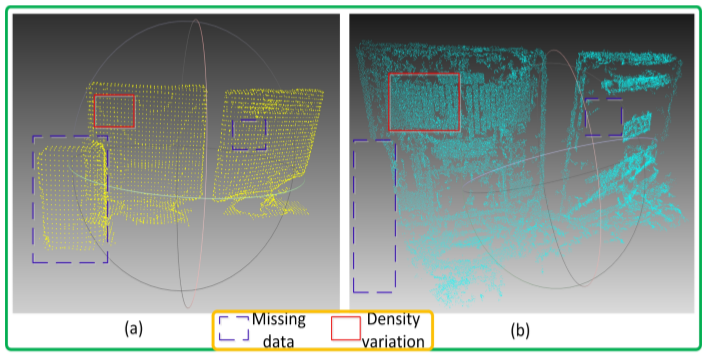
\includegraphics[width= \linewidth]{kinect.png}
  \caption{Difference in point density between Kinect (a) and a cloud reconstructed from multiple 2d RGB cameras (b). Illustration from \cite{huang:kinect}.}
  \label{fig:kinect}
\end{figure}

Mostly focused on point clouds obtained from these two sources: 1) Kinect; 2) reconstruction from multiple 2D RGB cameras.
\begin{algorithm}
\caption{Point Cloud Registration \cite{huang:kinect}}
\label{algo:kinect}
\begin{algorithmic}
  \REQUIRE two 3d point clouds
  \ENSURE registration of the two clouds
  \STATE normalize the scales of the two images
  \STATE supervoxel clustering: build a graph for each point cloud
  \STATE add features on each vertex by computed the ensemble shape function of its cluster of points
  \STATE find best matching between the two graphs
  \STATE remove mismatched vertices ("outliers") using ICP/RanSaC
  \STATE deduce the 3d transformation corresponding to the graph matching
  \RETURN the 3d transformation
\end{algorithmic}
\end{algorithm}
% Input images $\rightarrow$ Scale normalization $\rightarrow$ structure extraction $\rightarrow$ graph construction $\rightarrow$ optimization $\rightarrow$ transformation $\rightarrow$ result. See diagram p. 4. of that paper.

The micro and macro structure extraction consists in clustering voxels (3d pixels) into supervoxels. Look for the sourcecode of the clustering algorithm in the Point Cloud Library \cite{rusu:pclib}.
To solve the graph matching problem, see \cite{zhou:graphmatching, cour:graphmatching, zaslavskiy:graphmatching, frank:quadratic, gertz:ooqp}.

    \subsubsection{Point cloud registration with outliers \cite{papazov:rotations}}
Note that ICP amounts to searching for a rigid transformation $T$ which minimizes the sum of distances between closest points, for two pointclouds $D$ and $M$:
$$\sum_{x \in D} d(T(x),M)$$

Propose to search instead for a rigid transformation $T$ by minimising instead the sum: $$\sum_{x \in D}-\varphi(d(T(x), M))$$
where $-\varphi$ % $: \mathbb{R^+} \rightarrow \mathbb{R}$
is a function which is both increasing and bounded, satisfying $-\varphi(0) = -1$ and $\lim_{d \rightarrow +\infty} -\varphi(d) = 0$. The function $-\varphi$ becomes almost constant for large values of the distance $d$; hence points that are very badly matched cannot have a strong incidence on the minimisation. In a way, the algorithm proposed in this paper is a variant of ICP robust to outliers. It could also be used to detect and remove outliers?

The used formula for $\varphi$ is:
$$\varphi(d) = \frac{1}{1+\alpha d}$$
for some parameter $\alpha$.

The parameter $\alpha$ can be chosen as a function of two parameters $d_0$ and $\delta$ so that $\varphi(d) < \delta$ as soon as $d > d_0$, using the formula:
$$\alpha = \frac{1-\delta}{\delta {d_0}^2}$$
In their implementation, they choose $\delta = 0.1$ and set $d_0$ to $1/4$ of the minimum of the three dimensions of the bouding box of the point cloud.

This paper also gives very cool formulae to perform dichotomy on the space of 3d rotations, and to select "uniformly at random" rotations in this space or in the dichotomy subspaces.

  \subsection{Intensity-based registration}
    \subsubsection{Using intensity for the similarity measure}
Need to find more references about this.

Only useful if all images come from the same modality. Usually requires intensity normalization of the two images.
    \subsubsection{Electron microscopy to light microscopy \cite{acosta:intensity}}
Intensity-based registration, specific for 3d light microscopy (LM) to 3d electron microscopy (EM). The 3d images are stacks; in particular, the size of a pixel in the $z$-axis differs from the size in the $x$ and $y$ axes.

First, a translation is computed to pre-align the images in the $xy$-plane, because the misalignment in that plane is expected to be greater than in the $z$-axis. A 3d region of interest is selected in the stack, by human intervention or by some other algorithm. The light microscopy stack is projected into a 2d image using maximum-intensity projection, while a few slices are selected from the electron microscopy stack. Then each EM slice is aligned to the LM projection, using a rotation-invariant similiarity measure on a histogram-based description of the Laplacian-of-Gaussian of each of the two images. The full LM stack is shifted by a weighted average of the translations corresponding to each EM slice.

Second, a 2d affine transformation is computed to align the 3d LoG-EM-RoI and the pre-aligned 3d LoG-LM-RoI. The LoG-LM stack is resampled with a low-pass filter and a bilinear interpolator, so that pixel size for the two images are the same. The transformation is computed using the similarity measure Mutual Information, and is computed in two steps: first, a rigid transformation, ie, a direct isometry; then, an additional affine transformation.

  \subsection{Cross-modal registration using image analogies}
    \subsubsection{Generating an image looking like modality $B$ given an image coming from modality $A$ \cite{hertzmann:analogies}}See Fig. \ref{fig:analogies}.
\begin{figure}[h!]
  \centering
  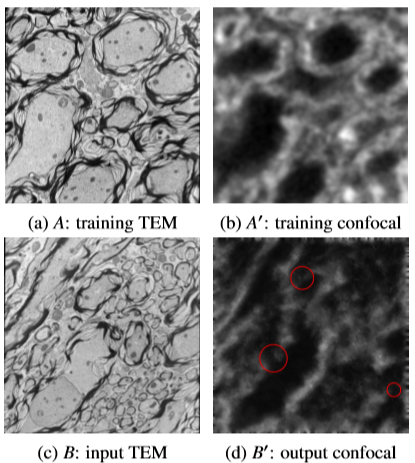
\includegraphics[width=0.60 \linewidth]{analogies.png}
  \caption{After training on pairs of images coming from two different modalities, the neural network can simulate an image from the second modality when given an image from the first modality. Illustration from \cite{cao:analogies}.}
  \label{fig:analogies}
\end{figure}
    \subsubsection{Building dictionaries of features \cite{cao:analogies}}
Uses machine learning on a training dataset of pairs of images from two different modalities to learn two dictionaries $D_A$ and $D_B$ of small filters for each modality.

To register an image $I_A$ from modality $A$ with an image $I_B$ from modality $B$: first, the image $I_A$ from modality $A$ is converted into a sparse vector $\alpha$ such that $I_A$ can be reconstructed from vector $\alpha$ and dictionary $D_A$. Then an image $I_B'$ is constructed from $\alpha$ and $D_B$. Then images $I_B$ and $I_B'$ can be registered using a uni-modality registration algorithm. See Fig. \ref{fig:dico}.
\begin{figure}[h!]
  \centering
  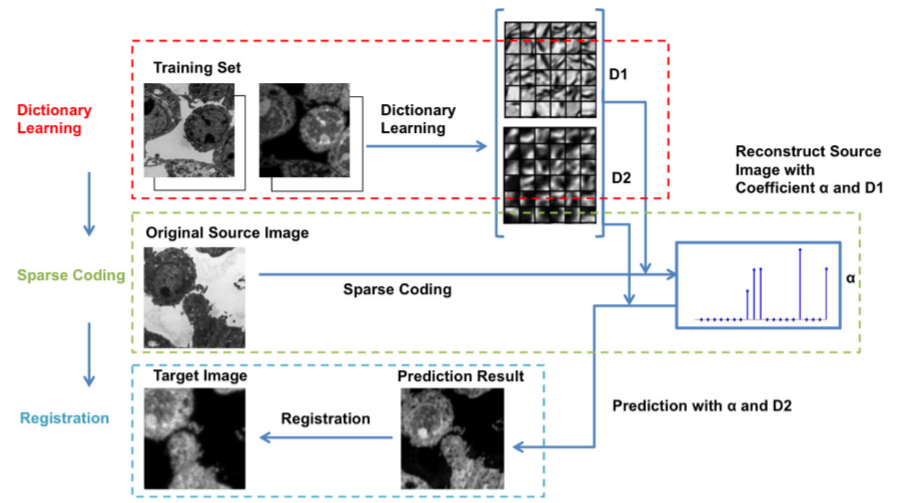
\includegraphics[width=\linewidth]{dico.png}
  \caption{Summary of the registration algorithm using deep learning to extract dictionaries of features. Illustration from \cite{cao:analogies}.}
  \label{fig:dico}
\end{figure}

\subsubsection{How to solve the registration problem with the reconstructed image}

\begin{enumerate}
  \item Denoising the image rebuilt from the dictionary of features \cite{elad:denoisingdico, li:denoisingdico} (note: surprisingly, \cite{cao:analogies} does not cite \cite{li:denoisingdico}) and denoising the target image
  \item ``We consider rigid followed by affine and B-spline registrations in this paper and use elastix’s implementation \cite{klein:elastix, ibanez:itk}. As similarity measures we use sum of squared differences (SSD) and mutual information
(MI). A standard gradient descent is used for optimization. For B-spline registration, we use displacement
magnitude regularization which penalizes ${||T (x) - x||}^2$,
where $T (x)$ is the transformation of coordinate $x$ in an
image \cite{klein:elastix}. This is justified as we do not
expect large deformations between the images as they
represent the same structure. Hence, small displacements are expected, which are favored by this form of
regularization.'' \cite{cao:analogies}
\end{enumerate}

  \subsection{Using similarity measures with deep learning \cite{litjens:deeplearning}}
    \subsubsection{Extracting features in MR brain images with unsupervised deep learning \linebreak[4] \cite{wu:features} }
Proposes an unsupervised deep learning approach to directly learn the basis filters that can effectively represent all observed image patches in magnetic resonance (MR) brain images. The coefficients by these learnt basis filters in representing the particular image patch can be regarded as the morphological signature for correspondence detection during image registration. Specifically, a stacked two-layer convolutional network is constructed to seek for the hierarchical representations for each image patch, where the high-level features are inferred from the responses of the low-level network.

Not multimodal: only MR images. But the training is unsupervised.

    \subsubsection{Using a convolutional neural network to compute the similarity measure in multi-modal registration \cite{simonovsky:crossmodalfeatures}}
Proposes a metric based on a convolutional neural network, to replace Mutual Information as a similarity measure. The network can be trained from scratch even from a few aligned image pairs. The metric is validated on intersubject deformable registration.

Supervised, but requires ``only a few'' aligned image pairs. Multi-modal?

    \subsubsection{Using stacked auto-encoders to compute the similarity measure in multi-modal registration \cite{cheng:deepsimilarity}}
Trains a binary classifier to learn the correspondence of two image patches. The classification output is transformed to a continuous probability value, then used as the similarity score. Proposes to utilise multi-modal stacked denoising autoencoder to effectively pre-train the deep neural network. Train and test the proposed metric using sampled corresponding/non-corresponding computed tomography and magnetic resonance head image patches from a same subject.

Multi-modal: MR and CT.

\section{Image segmentation}
\subsection{Cell segmentation}
See Fig. \ref{fig:cells}.
\begin{figure}[h!]
  \centering
  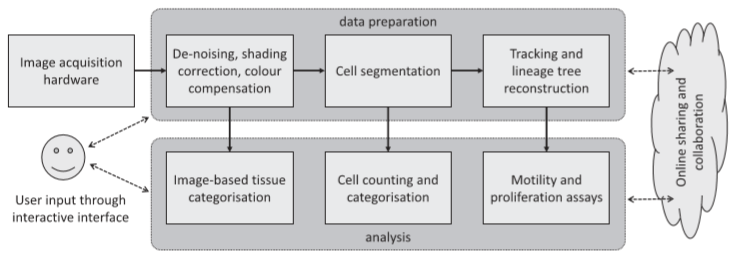
\includegraphics[width= \linewidth]{cells.png}
  \caption{Common tasks in analysis of cell images. Illustration from \cite{kan:machine}.}
  \label{fig:cells}
\end{figure}
    \subsubsection{Colour threshold and pixel adjacency}
Apply filters to remove noise, blur, and non-cell objects. Use an intensity threshold to classify pixels as part of a cell or part of the background. Use connected component analysis to separate non-touching cells. If cells overlap, use a ``watershed'' technique to separate them.

    \subsubsection{After segmentation, decision tree to classify an image segment as a cell or not a cell based on its area and elongation \cite{kan:machine}}
After segmenting the objects in the image, classify each object as a cell or not a cell. Possible features for the classifier:
\begin{itemize}
  \item area (small objects are not cells);
  \item elongation $4 \pi A / P^2$, where $A$ is area and $P$ is perimeter (close to 1 if object is shaped like a disc, close to 0 if it is shaped like a line).
\end{itemize}

    \subsubsection{Convolutional neural networks}
       \paragraph{2018 Data Science Bowl \cite{marks:bowl}}
A contest on kaggle to devise algorithms for cell segmentation. The algorithms are required to be able to handle images from several different experiments using light microscopy. The three best ranked submissions to the contest use convolutional neural networks and perform significantly better than the software CellProfiler, while not requiring the user to spend time configuring the software. The good performance of these solutions appears to come in particular from the succesful use of data augmentation and data preprocessing. See Fig. \ref{fig:bowl}.
\begin{figure}[h!]
  \centering
  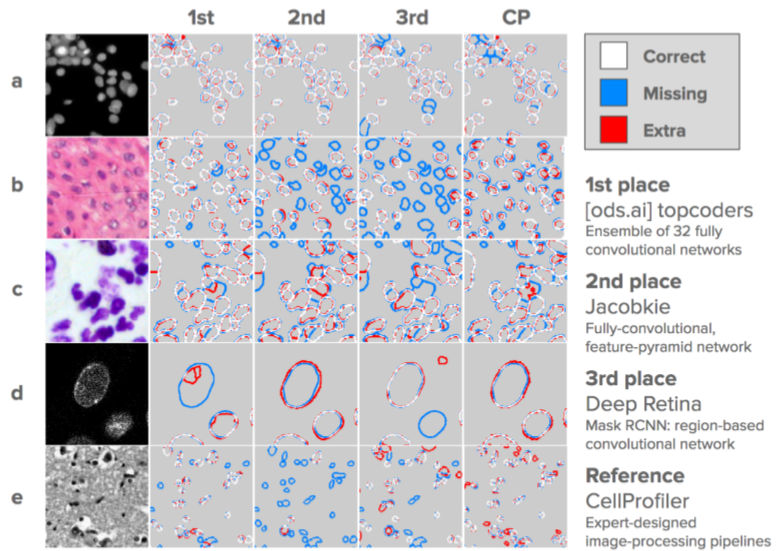
\includegraphics[width= \linewidth ]{bowl.png}
  \caption{Illustration from \cite{marks:bowl}.}
  \label{fig:bowl}
\end{figure}



    \subsubsection{Tracking and constructing lineage trees}
Cells are observed over time. Need to track individual cells over time. Cells might overlap in some frames; a cell might divide through mitosis.
    \paragraph{Classification problem over two successive segmented frames}
Given two successive frames, classify all pairs (cell from first frame, cell from second frame) as ``same cell'' or ``distinct cells'' \cite{kan:machine}. See Fig. \ref{fig:tracking}.

\begin{figure}[h!]
  \centering
  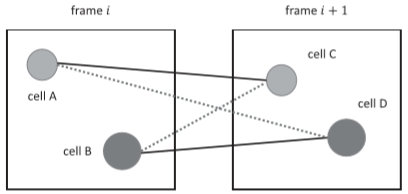
\includegraphics[width=.75 \linewidth ]{tracking.png}
  \caption{Illustration from \cite{kan:machine}.}
  \label{fig:tracking}
\end{figure}

  \subsection{Pixel classification}
    \subsubsection{IlastiK~\cite{berg:ilastik}}
      A program in python which implements supervised pixel classification, as well as a few other segmentation problems. The algorithm for pixel classification in IlastiK is described in Algorithm~\ref{algo:ilastikpixel}.
      \begin{algorithm}
      \caption{IlastiK Pixel Classification~\cite{berg:ilastik}}
      \label{algo:ilastikpixel}
      \begin{algorithmic}
        \REQUIRE an image or a sequence of images
        \ENSURE classification of each pixel in the images
        \STATE Choose a set of predefined convolutional filters, such as edge detection or Laplacian of Gaussian
        \STATE Compute features for every pixel
        \STATE Ask the user to "paint" some pixels with a label, using a paintbrush
        \STATE Build a random forest using the computed features for each pixel and the user-provided labels
        \STATE Apply the random forest to every pixel in the image
        \STATE Show the classification result to the user; ask them to paint some labels again to improve classification
        \STATE Loop until the user is satisfied with the classification
        \RETURN the whole pixel classifier, features + random forest, to be applied directly to other images
      \end{algorithmic}
      \end{algorithm}
      The program provides a paintbrush-like interface to "paint" some pixels to mark them with a training label. 3d images can be viewed by slices along three axes. There is a two-step variant of pixel classification based on Tu and Bai's autocontext algorithm~\cite{tubai:autocontext}. IlastiK also provides a few other functionalities, such as object classification, or tracking of moving segmented objects across frames.


\section{Other applications of deep learning in medical imaging \cite{litjens:deeplearning}}
  \subsection{Classification of images from medical exams}
  \subsection{Content-based image retrieval}
    Browsing massive databases, for instance retrieving similar case histories. Feature extraction is very useful here.
  \subsection{Generating text reports from images \cite{schlegl:text}}











%
%
%\section{Crocoval}
%
%\section{ICP
%\cite{besl:icp, chen:icp}}
%Presents the Iterative Closest Point algorithm, to register two 3d shapes.
%
%\section{Random sample consensus
%\cite{fischler:ransac}}
%Presents the RanSaC algorithm.
%\begin{itemize}
%  \item \emph{Input:} a set of $N$ points; a model that requires $n < N$ points to instantiate; a tolerance threshold $\alpha$; a number of points threshold $t$
%  \item Loop:
%  \begin{itemize}
%    \item Select $n$ points at random
%    \item Instantiate the model using these $n$ points
%    \item Find all points that fit the model with a tolerance error $\leq \alpha$
%    \item If the number of points is at least $t$:
%    \begin{itemize}
%      \item Use all these points to fit a new model
%      \item Terminate and return the new model
%    \end{itemize}
%    \item End if.
%  \end{itemize}
%  \item End loop.
%\end{itemize}
%
%
%\section{Point cloud registration
%\cite{huang:kinect}}
%
%
%Proposes an algorithm for registration of 3d clouds of points, with more than a thousand points: possibly tens of thousands or millions of points. The two clouds may have been generated using different kinds of sensors, and thus present differences, such as inequal point density or missing parts of the represented object. The idea behind the algorithm is to extract the "macro" and "micro" structures from the images, and use them to build a graph for each image representing those structures. The point cloud registration problem becomes a graph matching problem. The structure extraction algorithm is adapted from a previous paper \cite{papon:supervoxels}.
%
% Input images $\rightarrow$ Scale normalization $\rightarrow$ structure extraction $\rightarrow$ graph construction $\rightarrow$ optimization $\rightarrow$ transformation $\rightarrow$ result. See diagram p. 4. of that paper.
%
%Mostly focused on point clouds obtained from these two sources: 1) Kinect; 2) reconstruction from multiple 2D RGB cameras.
%
%\section{Registration using image analogies
%\cite{cao:analogies}}
%
%Uses machine learning on a training dataset of pairs of images from two different modalities to learn two dictionaries $D_A$ and $D_B$ of small filters for each modality.
%
%To register an image $I_A$ from modality $A$ with an image $I_B$ from modality $B$: first, the image $I_A$ from modality $A$ is converted into a sparse vector $\alpha$ such that $I_A$ can be reconstructed from vector $\alpha$ and dictionary $D_A$. Then an image $I_B'$ is constructed from $\alpha$ and $D_B$. Then images $I_B$ and $I_B'$ can be registered using a uni-modality registration algorithm. See Fig. 3 p. 4 in the paper.
%
%
%\section{Future of CLEM
%\cite{perrine:future}}
%
%
%\section{Intensity-based matching
%\cite{acosta:intensity}}
%
%Intensity-based registration, specific for 3d light microscopy to 3d electron microscopy. The 3d images are stacks; in particular, the size of a pixel in the Z-axis differs from the size in the X and Y axes.
%
%First, the images pre-aligned in the XY-plane, because the misalignment in that plane is expected to be greater than in the Z-axis. A 3d region of interest is selected in the stack, by human intervention or by some other algorithm. The light microscopy stack is projected into a 2D image using maximum-intensity projection, while a few slices are selected from the electron microscopy stack. Then each EM slice is aligned to the LM projection, using a rotation-invariant similiarity measure on a histogram-based description of the Laplacian-of-Gaussian of each of the two images. The full LM stack is shifted by a weighted average of the translations corresponding to each EM slice.
%
%Second, a 2d affine transformation is computed to align the 3d LoG-EM-RoI and the pre-aligned 3d LoG-LM-RoI. The LoG-LM stack is resampled with a low-pass filter and a bilinear interpolator, so that pixel size for the two images are the same. The transformation is computed using the similarity measure Mutual Information, and is computed in two steps: first, a rigid transformation, ie, a direct isometry; then, an additional affine transformation.
%
%
%\section{Multi-modal registration 2d 3d
%\cite{acosta:these}}
%
%
%\section{Machine-learning and cells
%\cite{kan:machine}}
%A brief survey on applications of machine learning to the analysis of images of cells acquired with light microscopy, for instance segmenting, tracking, constructing lineage trees.
%%\begin{itemize}
%%  \item Decision tree to classify an image segment as a cell or not a cell based on its area and elongation;
%%  \item Given two successive frames, classify all pairs (cell from first frame, cell from second frame) as "same cell" or "distinct cells";
%%\end{itemize}
%
%
%
%\section{Data Science Bowl
%\cite{marks:bowl}}
%
%A contest on kaggle to devise algorithms for cell segmentation. The algorithms are required to be able to handle images from several different experiments using light microscopy. The three best ranked submissions to the contest use convolutional neural networks and perform significantly better than the software CellProfiler, while not requiring the user to spend time configuring the software. The good performance of these solutions appears to come in particular from the succesful use of data augmentation and data preprocessing.
%
%
%\section{New insights on mitral valve: Filamin-A
%\cite{letourneau:filamina}}


\bibliographystyle{apalike}
\bibliography{summaries}

\end{document}
